\chapter{Learning structure without supplied targets}
\label{ch:unsupervised-learning}

\begin{learningobjectives}
After this chapter, you should be able to:
\begin{itemize}
  \item distinguish clustering, dimensionality reduction, density estimation,
  anomaly detection, and graph representation by their mathematical outputs;
  \item specify the representation, geometry, and validation claim of an
  unsupervised analysis;
  \item explain how scaling and relational construction change the learned result;
  \item separate internal evidence, stability evidence, and external scientific audits; and
  \item design an unsupervised software artifact with reproducible fitted state.
\end{itemize}
\end{learningobjectives}

\begin{chapterconnection}
Part II began with a target $Y$ and asked how observations $X$ could support
prediction under a stated future-use contract. Part III begins when a useful
target is unavailable, delayed, contested, or deliberately withheld. The
absence of $Y$ does not remove assumptions. It moves them into representation,
distance, neighborhood, topology, objective, and validation.
\end{chapterconnection}

\section{From prediction to structure}

In supervised learning, an empirical objective compares model output with a
provided target. In unsupervised learning, the algorithm receives observations
$X=(x_1,\ldots,x_n)^\top$, relations $A$, or both, and returns a structural
object. That object may be a partition, a density, a low-dimensional coordinate
system, a reconstruction, a set of communities, or an anomaly score.

The phrase \emph{without labels} is therefore incomplete. One should ask:
without which labels, for which population, under which observation process,
and toward which structural objective? Patient identifiers, acquisition sites,
time stamps, and later outcomes may still exist. They can diagnose confounding
or support an external audit even when they are not supplied to fitting.

\begin{center}
  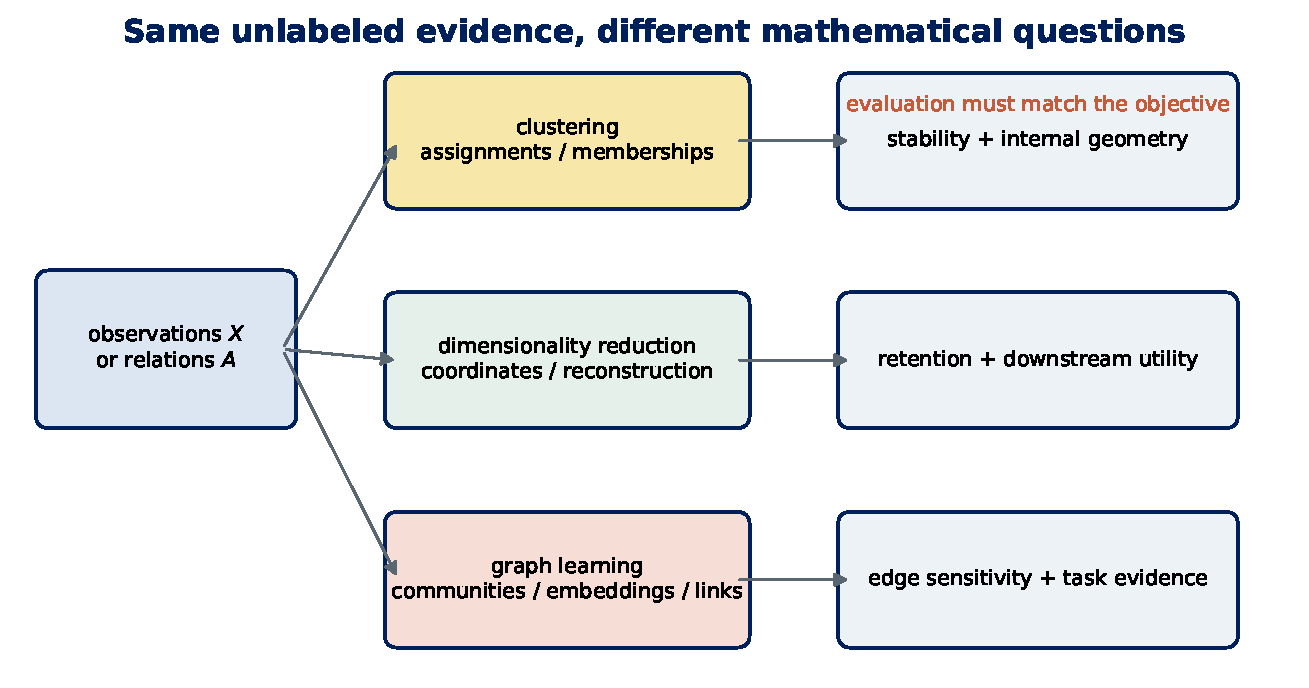
\includegraphics[width=0.98\textwidth]{figures/generated/unsupervised-task-map.pdf}
\end{center}

The three branches in the figure consume related evidence but answer different
questions. A good two-dimensional embedding need not yield a good partition. A
well-separated partition need not be scientifically meaningful. A graph
community depends on which relations became edges.

\section{A taxonomy by output and invariance}

\textbf{Clustering} returns assignments $c_i$, membership probabilities, or a
hierarchy. Its invariances include arbitrary relabeling of cluster identifiers:
cluster 0 and cluster 2 can be exchanged without changing the partition.

\textbf{Dimensionality reduction} returns a map
$f:\mathbb{R}^p\rightarrow\mathbb{R}^k$, usually with $k<p$, and sometimes an
inverse or reconstruction map. Different methods preserve different objects:
global variance, pairwise distance, local neighborhoods, angles, or likelihood.

\textbf{Density estimation} returns an estimated probability density or mass
function. \textbf{Anomaly detection} returns a score relative to a reference
population; an unusual observation is not necessarily erroneous or harmful.

\textbf{Graph learning} begins with nodes and edges. It may return communities,
node or graph embeddings, link scores, diffusion behavior, or reconstructed
relations. A feature table treats rows as separate observations; a graph makes
dependence part of the input.

\textbf{Self-supervised learning} creates a supervised signal from the data:
mask a token, predict a transformed view, or contrast paired and unpaired
examples. The pretext task is not usually the final scientific task. It is a
mechanism for learning a reusable representation.

\conceptcheck{A method maps spectra to two coordinates and a scientist then
runs $K$-means in those coordinates. Which two objectives have been composed?
What evidence would be needed for each?}

\section{Representation is part of the hypothesis}

Suppose a row contains mass in grams, temperature in kelvin, and a dimensionless
ratio. Euclidean distance is
\[
d(x_i,x_j)^2=\sum_{r=1}^{p}(x_{ir}-x_{jr})^2.
\]
Changing a unit changes that geometry. Standardization,
\[
z_{ir}=\frac{x_{ir}-\bar x_r}{s_r},
\]
encodes a policy that a one-standard-deviation change is comparable across
features. It is not a unit-free fact about nature. Robust scaling may be more
appropriate under contamination; known measurement uncertainties may motivate
a weighted metric; compositional or directional data require different
geometry.

Mixed numerical and categorical features, missingness, repeated measurements,
time, and spatial dependence likewise require explicit representation choices.
One-hot encoding followed by ordinary Euclidean distance gives category
differences a particular weight. Mean imputation can manufacture dense central
regions. Treating repeated measurements as independent nodes can cause subject
identity to dominate the discovered structure.

\begin{professionalbox}
Version the raw schema, selected variables, units, transformation state,
distance or kernel, fitted algorithm, seed, and software release. A cluster
assignment file without this provenance is not a reproducible scientific
artifact.
\end{professionalbox}

\section{K-means as a precise example}

For $K$ nonempty groups, $K$-means minimizes within-cluster squared Euclidean
distance:
\begin{equation}
\label{eq:kmeans-objective}
J(c,\mu)=\sum_{i=1}^{n}\lVert x_i-\mu_{c_i}\rVert_2^2,
\qquad c_i\in\{1,\ldots,K\}.
\end{equation}

Given centroids, each observation is assigned to its closest centroid. Given
assignments, each centroid is updated to the mean of its assigned observations.
These two steps alternate until a stopping rule is met.

\begin{theorem}[the mean minimizes within-cluster squared distance]
\label{thm:kmeans-centroid}
For nonempty vectors $x_1,\ldots,x_m\in\mathbb{R}^p$, the function
$Q(a)=\sum_{i=1}^{m}\lVert x_i-a\rVert_2^2$ is uniquely minimized by
$a=\bar x=m^{-1}\sum_i x_i$.
\end{theorem}

\begin{proof}
Write $x_i-a=(x_i-\bar x)+(\bar x-a)$. Expanding and summing gives
\[
Q(a)=\sum_i\lVert x_i-\bar x\rVert_2^2
+m\lVert a-\bar x\rVert_2^2
+2(\bar x-a)^\top\sum_i(x_i-\bar x).
\]
The last term is zero. The first is independent of $a$, and the second is
nonnegative with equality only at $a=\bar x$.
\end{proof}

Each alternating step cannot increase Equation~\eqref{eq:kmeans-objective}, but
the objective is nonconvex in assignments and centroids jointly. Initialization
can lead to different local solutions. Repeated initializations address one
numerical sensitivity; they do not answer whether spherical, similarly scaled
clusters are an adequate model of the science.

\begin{misconceptionbox}
\textbf{Misconception:} the elbow in an inertia plot reveals the true number of
clusters. \textbf{Correction:} inertia decreases whenever $K$ increases and is
zero when every distinct observation receives its own centroid. An elbow is a
judgment about marginal compression under this geometry, not a theorem that a
population has $K$ natural kinds.
\end{misconceptionbox}

\section{Validation without a training target}

Unsupervised evaluation must be attached to a claim.

\textbf{Internal evidence} uses the fitted representation and geometry.
Silhouette compares within-cluster cohesion with nearest-cluster separation.
The $K$-means objective measures compactness. These can diagnose the stated
objective, but cannot establish external meaning.

\textbf{Stability evidence} perturbs observations, features, initialization,
hyperparameters, or time windows and compares results. Because cluster codes
are arbitrary, assignments must be aligned or compared with permutation-
invariant measures. Instability may reflect weak structure, finite samples, or
an algorithm near a boundary.

\textbf{External evidence} compares a learned structure with information not
used to fit or select it: a later phenotype, expert assessment, intervention,
or known category. The adjusted Rand index compares pairs of assignments while
correcting its expectation under a chance model. External disagreement does
not automatically make the clustering useless; it may reveal that the
algorithm preserved a different axis of variation. Agreement does not prove a
causal or ontological discovery.

\textbf{Downstream evidence} asks whether the representation helps a separate
task under honest evaluation. That task may be prediction, retrieval,
compression, visualization, or experimental design. Once labels select the
representation, the combined procedure is supervised or semi-supervised and
must be evaluated as such.

\section{Graph and relational evidence}

Let $G=(V,E)$ be a graph with $n$ nodes. An adjacency matrix $A\in\mathbb{R}^{n
\times n}$ records relations; a degree matrix $D$ has
$D_{ii}=\sum_j A_{ij}$; and an unnormalized graph Laplacian is
\[
L=D-A.
\]
For every $u\in\mathbb{R}^n$ in an undirected weighted graph,
\begin{equation}
\label{eq:laplacian-energy}
u^\top Lu=\frac12\sum_{i,j}A_{ij}(u_i-u_j)^2\ge 0.
\end{equation}
Thus low-energy vectors change slowly across strong edges. Spectral clustering
and graph embeddings use eigenvectors associated with small nontrivial
Laplacian eigenvalues to expose such structure.

Equation~\eqref{eq:laplacian-energy} makes the assumption visible: connected
nodes are encouraged to have similar coordinates. In a molecular bond graph
that may be useful; in a social network with adversarial, transactional, or
heterophilous relations it may be wrong. Direction, edge type, weight, time,
and missing edges matter.

A graph can also be constructed from a feature table, for example by joining
each observation to its $k$ nearest neighbors. That construction is itself a
model. Scaling, metric, $k$, mutual versus one-sided neighbors, and symmetrizing
rules all change $A$ before a graph algorithm begins.

\section{Worked example: chemistry, clusters, and relations}

The UCI Wine data contain thirteen chemical measurements for 178 wines from
three cultivars. A defensible exploratory workflow is:
\begin{enumerate}
  \item query the versioned observations and inspect ranges, missingness, and provenance;
  \item exclude identifiers and cultivar labels from the learning matrix;
  \item state and fit a scaling policy;
  \item fit $K$-means under several seeds and values of $K$;
  \item report inertia, silhouette, and assignment stability;
  \item use the withheld cultivar only as an external audit; and
  \item construct several neighbor graphs and test whether conclusions survive
  reasonable edge definitions.
\end{enumerate}

The result is not ``three cultivars were discovered.'' A precise report states
that, under a standardized Euclidean representation and a compact-centroid
objective, one fitted partition aligned to a quantified degree with a withheld
cultivar annotation. It then records sensitivities and plausible alternative
explanations such as chemical variables dominated by production conditions.

\begin{workedexample}{when labels enter after fitting}
A laboratory has batch labels and a later biological assay. It withholds both,
clusters standardized spectra, and measures bootstrap stability. Batch labels
are then revealed: one stable cluster is almost entirely a single instrument
batch. The biological assay shows little separation.

The cluster is reproducible but not biologically useful. The analysis has still
found an important result---a batch effect that must be corrected or designed
around. Calling the cluster a phenotype would have confused stability with
meaning.
\end{workedexample}

\section{Engineering the fitted artifact}

An unsupervised estimator needs the same public discipline as a supervised
one. Its API specifies input shape, numeric policy, randomness, convergence,
fitted attributes, transform or prediction behavior, and failure modes. Tests
should cover analytic cases, invariances, invalid values, fitted-state checks,
reproducibility, and comparison with a trusted implementation.

Do not make a notebook the only copy of a clustering or decomposition
algorithm. The notebook poses questions, displays evidence, and interprets
results. Reusable fitting and transformation belong in a package; behavior
contracts belong in tests; repeated batch work belongs in scripts; CI checks
the source; and a stored artifact includes preprocessing state.

Monitoring must follow the output. For clustering, track input schema and
population, distance-to-centroid distributions, cluster prevalence, and
unassigned or low-confidence cases. For embeddings, track reconstruction or
neighborhood evidence and coordinate conventions. Cluster numbers and component
signs may change without semantic change, so naive coordinate-by-coordinate
alerts can be false alarms.

\section{Exercises}
\begin{enumerate}
  \item \textbf{Intuition.} Give two datasets with the same rows for which two
  scientifically defensible unit choices produce different nearest neighbors.
  State which question makes each choice defensible.
  \item \textbf{Mathematics.} Prove Equation~\eqref{eq:laplacian-energy} for a
  symmetric adjacency matrix and characterize when the energy is zero.
  \item \textbf{Clustering.} Use Theorem~\ref{thm:kmeans-centroid} to show that
  each centroid-update step cannot increase the $K$-means objective.
  \item \textbf{Evaluation.} Design internal, stability, external, and downstream
  evidence for clustering cells from gene-expression measurements.
  \item \textbf{Graph sensitivity.} Compare $k$-nearest-neighbor graphs for
  several $k$ values. Report connected components, degree distribution, and one
  conclusion that is stable across the range.
  \item \textbf{Contribution.} Propose a clusterer or graph transformer for the
  course package. Write its typed interface, NumPy-style docstring outline, two
  analytic invariants, three failure tests, and trusted-reference comparison.
  Open an issue before implementation and link the final PR to that issue.
\end{enumerate}

\begin{chapterreview}
Unsupervised learning replaces a supplied target with a structural objective;
it does not remove modeling choices. Clustering, dimensionality reduction,
density, anomalies, and graph methods return different objects and require
different evidence. Representation and scaling define geometry. Internal
scores measure the chosen objective, stability measures sensitivity, and
external or downstream evidence supplies meaning. Reproducible fitted state and
software contracts remain part of the scientific claim.
\end{chapterreview}

\begin{notebooklink}
Lecture 16 notebook 00 uses real wine chemistry to connect clustering,
dimensionality reduction, and a nearest-neighbor graph. It keeps cultivar labels
outside fitting and uses them only for an explicit external audit.
\end{notebooklink}
